\documentclass{svproc}
\usepackage{url}
\usepackage{cite}
\usepackage[ruled,vlined]{algorithm2e}
\usepackage{graphicx}
\usepackage{amsmath}
\usepackage{amssymb}
\usepackage{algpseudocode}
\usepackage{todonotes}

\def\UrlFont{\rmfamily}


\begin{document}
    \mainmatter
    \title{Analysis of Artificial Intelligence Strategies\\On The Game 2048
    }
    \subtitle{CS7IS2 Project (2019/2020)}
    \author{Rohan Anand, Rohan Bagwe, Sameer Karode, Kavithvajen Kamaraj}

    \institute{Trinity College Dublin \newline
        \email{anandr@tcd.ie}, \email{bagwer@tcd.ie}, \email{karodes@tcd.ie}, \email{kamarajk@tcd.ie}}

    \maketitle

    \begin{abstract}
        \todo{update abstract}
        Video games and puzzle problems have become popular when researching reinforcement learning techniques in Artificial Intelligence. In our paper, we analyze the performance of multiple agents in 2048, a popular puzzle-like game. These agents are trained using Monte-Carlo search, Expectimax, and Q-learning. The results of these experiments indicate that BLANK method works best for this game. This could be due to ... (reasoning to be given later)
        \keywords{Artificial Intelligence, 2048 Game, DQN, Monte Carlo Tree Search, Expectimax}
    \end{abstract}

    \section{Introduction}

    \todo{update Intro :In this section, you should introduce your work: what are the motivations behind this work? What is the relevant problem that you are investigating? Why is it relevant?
    Briefly, introduce the background information required to understand the problem and the concepts that you will develop.}

    - Games have been important in research in Artificial Intelligence, especially in the area of reinforcement learning. (Why?)
    - Deepmind winning chess, go, shoji
    - Starcraft, DOTA AIs

    - Many reinforcement learning algorithms have been tested using games such as atari. (Talk about these researches)
    In this paper we take a look at reinforcement learning for the game 2048. The goal of the game is to form a block with the highest number possible.
    - We implement 3 algorithms on the game environment: (Name the algos). The relative performance of these algorithms is then measured and evaluated.

    Every game is modeled as a search problem with a heuristic evaluation function. This enables an AI agent to find the optimum solution for solving the game.
    \section{Related Work}

    \todo{In this section you will discuss possible approaches to solve the problem you are addressing, justifying your choice of the 3 you have selected to evaluate. Also, briefly introduce the approaches you are evaluating with a specific emphasis on differences and similarities to the proposed approach(es).

    }
    Expectimax is a recursive depth-limited tree search algorithm that does not treat the game as adversarial \cite{Maryam}. Adversarial search is performed in an multi-agent environment where two agents play against each other and try to explore and evaluate the shared search space for the solution ahead of each other. An agent decides the move to be played by playing all response moves of the opponent concerning every possible move of the agent. The most common example is the Mini-Max algorithm \cite{7162574, Dan} that uses an adversarial search to evaluate each move in terms of loss and gain for one of the agents. Each agent evaluates the search space such that the opponent agent gets the minimum benefit thereby increasing their reward. adversarial Search is widely used in the Zero-sum games such as tic-tac-toe where each agent has complete information about the game’s state. However, this approach is not suitable for creating an AI agent to play the 2048 game as the knowledge of the game is not perfect. Each time a new random tile is generated from a probability distribution with 90\% chances of generating a 2-tile and 10\% chances of generating a 4-tile in an empty cell of the board. Since the tiles spawned are at random, they are not necessarily targeted to the worst empty cell on the board. In Expectimax search, at every state of the game board, the maximum expected utility \cite{Maryam} chooses the next move to be played with a maximum fitness value calculated through averaged depth limit search weighted by the probability of occurrence of that state (p=0.9 for 2-tile and p=0.1 for 4-tile) and a heuristic function. In Expectimax search, the chance nodes are administered by probabilities instead of choosing the maximum and minimum nodes in the case of the Mini-Max algorithm \cite{7162574}.

    \section{Problem Definition and Algorithm} \label{Game Explanation}

    2048 is a non-deterministic, single-player game that was developed by a 19-year old web developer named Gabriele Cirulli. The game was released to the public in 2014 as a free and open-source software, and it quickly became the most popular game in the market when mobile versions of the game were released \cite{wiki_2048}. The game is interesting due to its simple controls and yet hard to master gameplay. One cannot simply win a game of 2048 by making random moves unless they’re very lucky. The game requires the player to have some sort of intelligence and an ability to look ahead of moves to determine what would lead them to go on and win the game, thus making it a perfect problem for an AI agent to solve. Also, 2048 can be clearly shown as a Markov Decision Process and that provides an ideal platform to compare and contrast different AI reinforcement learning techniques \cite{jaskowski, pedagogy}.

    % The 2048 game is played on a 4x4 grid where numbered tiles are present. The game randomly generated tiles with the numbers 2 and 4 after every move the player makes. The goal is to sum up similar tiles with one another until 2048 is reached in at least one tile. An example would be to add two tiles with the values 2 and they’d add up to become one tile with the value 4, now this tile with the value 4 must be added up with another tile with the value 4 to form a single tile with value 8, this goes on until two 8s are added to form 16 and so on until 2048 is reached. The rules of the game are very easy to understand but playing the game smartly in a constrained 4x4 grid is what is challenging about this game. The tiles are added by moving them either up, down, left or right and when one of the moves are performed all the tiles in the grid move in the specified direction. There is another element involved in this game and that is the score, it starts off at zero and as the player makes moves, it is updated based on the value of the new tiles that are formed due to the combination of previous tiles (i.e., if two tiles with the value of 128 are combined, then the resulting tile will have the value of 256 and thus the score will also increment by 256 points). A player wins when they obtain a tile with the value 2048, but the game does not end then and the users can continue the game to reach higher scores like 4096 and so on. The player is considered to have lost when all the tiles in the grid have a value and a move cannot be made to combine any of them.

    This project aims to demonstrate how various Reinforcement Learning algorithms perform while trying to win a game of 2048. The algorithms that were implemented are discussed in the later sections.

    \subsection{Random Moves Algorithm}

    This project started off with implementing an agent which randomly makes a move on game board out of 4 choices. It plays until the game is over. This is done several times while keeping track of the end game score. As this implementation is completely based upon random actions, the score serves as a baseline for evaluating rest of the other algorithms implemented in this project.

    % I dont think so???
    % Further, incremental improvements have been made so that agent can make informed decisions which will lead to a good score at the end of the run.

    \begin{algorithm}[h!]
        \SetAlgoLined
        initialize\_gamegrid()\;
        \While{game\_over != True}{
            random\_move = get\_random\_move()\;
            gamegrid.play(random\_move);
        }
        \caption{Random Moves Algorithm}
    \end{algorithm}

    \subsection{Greedy First Algorithm}
    In this approach, an agent makes a move which is likely to generate a higher game score against a particular action. For instance, if the agent has 4 choices, it calculates the new game score for all the viable choices and then chooses an action which corresponds to the highest score. Sometimes it might happen that all the moves are generating the same score, as there is no merging of tiles happening in a particular state. In such cases the agent will randomly choose a move out of allowed choices.

    \begin{algorithm}[h!]
        \SetAlgoLined
        initialize\_gamegrid()\;
        \While{game\_over != True}{
            score\_list = new list()\;
            \For{action in actions}{
                score\_for\_action = get\_score\_for\_move(action)\;
                score\_list.append(score\_for\_action)
            }
            index =  get\_max\_score\_index(score\_list)\;
            max\_score\_move = get\_corresponding\_move\_for(index)\;
            gamegrid.play(max\_score\_move);
        }
        \caption{Greedy First Algorithm}
    \end{algorithm}

    Several heuristics are used to direct the optimization algorithm towards favourable positions. The precise choice of a heuristic has a huge effect on the performance of the algorithm. The various heuristics are weighted and combined into a positional score, which determines how ``good'' a given board position is. The choice of heuristics are as follows:

    \begin{itemize}
        \item \textbf{{Max Score generated by immediate Move}}
        Using this heuristic agent can find the best move from a given set of actions based on the maximum score achieved. The calculation of score for the 2048 game is described in Section \ref{Game Explanation}.
        % Mathematically, equation for finding best move can be stated as follows.
        % \begin{equation} \label{max_score_equation}
        %              best\_move = argmax(score\_list\_of\_each\_move)
        % \end{equation}


        \item {\textbf{Number of Empty cells on game board after performing a move}}

        It takes into account the number of free tiles left. If there are few numbers of free available tiles, then it’s likely that the game will end with low premature scores. This heuristic tries to ensure that the player AI agent chooses the move that allows more free spaces by looking ahead. There is a penalty for having too few free tiles, since options can quickly run out when the game board gets too cramped.

        \item {\textbf{Weight Matrix Multiplication Score}}
        It has been observed that the agent can score well if the tiles with large values are maintained in the corner of the game grid \cite{blog_2048_weight_matrix}. By multiplying a weight matrix to game board, we can mimic this strategy by setting the values of \textbf{W} such that the weight decreases from the top left to the bottom right.

        \begin{equation}
            \textbf{W} =
            \begin{pmatrix}
                7 & 6 & 5 & 4 \\
                6 & 5 & 4 & 3\\
                5 & 4 & 3 & 2 \\
                4 & 3 & 2 & 1 \\
            \end{pmatrix}
        \end{equation}

        \begin{equation} \label{weighted_score_equation}
        \textbf{ weighted\_cell\_score} = \textbf{W} \times \textbf{game\_grid\_matrix}
        \end{equation}

        The equation \ref{weighted_score_equation} demonstrates that, the agent will tend to make moves such that the bigger tiles are always closer to the corner than the smaller tiles, which agrees with the desired strategy.The above weight matrix may not be the most ideal, it only helps illustrate the choice of the underlying heuristic. It is possible to use other optimization methods, such as Genetic Algorithms and Particle Swarm Optimization (PSO), which is currently out of scope of this paper.

        % \item {\textbf{Monotonicity property}}
        % This heuristic tries to ensure that the values of the tiles are all either increasing or decreasing along both the left/right and up/down directions. This heuristic alone captures the intuition that many others have mentioned, that higher valued tiles should be clustered in a corner. It will typically prevent smaller valued tiles from getting orphaned and will keep the board very organized, with smaller tiles cascading in and filling up into the larger tiles. A perfectly monotonic grid looks like figure \ref{fig:monotonicity}.

        % \begin{figure}[h!]

        %     \centering
        %     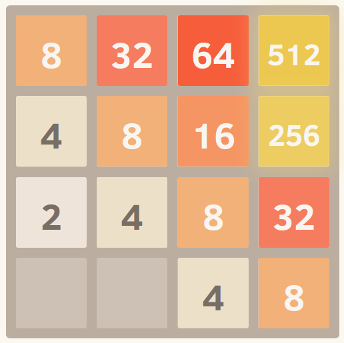
\includegraphics[width=0.15\textwidth]{monotonicity_2048.png}
        %     \caption{Demonstration of a monotonic grid}
        %     \label{fig:monotonicity}
        % \end{figure}

    \end{itemize}


    \subsubsection{Implementing Heuristics}
    In this project, implementation of the first three heuristics namely Max Score generated by immediate Move, Number of Empty cells, and weight matrix multiplication is done and its behavior is studied in greedy algorithm as well as Monte Carlo Tree Search. The algorithm can be updated with the following expression to accommodate heuristic score while computing next move.

    \begin{multline} \label{heuristic_score_equation}
    Heuristic \ Score  = \alpha \times Max \ Score \ of \  Immediate \ Move \\
    + \beta \times Number \ of \ Empty \  Cells \\
    + \gamma \times Weighted \ Matrix \ Multiplication \ Score  + K
    \end{multline}

    In equation \ref{heuristic_score_equation} \(\alpha ,  \beta , \gamma , and K \) are coefficients which helps tune the heuristic function. The combination of these parameters results in weighted heuristic function which can be used to study variation in performance of algorithms.

    \subsection{Monte-Carlo Tree Search (MCTS)}

    MCTS is a heuristic search algorithm that is widely used to solve Reinforcement Learning problems. Hence, MCTS can find its own moves and explore the environment on its own by randomly playing different moves \cite{mcts_comparison}. The following steps are followed in an iterative fashion to learn the policy of the problem \cite{mcts_medium}.

    \begin{algorithm}[h!]
        \SetAlgoLined
        Const TREE\_SEARCH\_DEPTH\;
        initialize\_gamegrid()\;
        \While{game\_over != True} {
            score\_list = new list()\;
            \For{action in actions}{
                scores = gamegrid.play(action)\;
                i = TREE\_SEARCH\_DEPTH\;
                \While{i less than 0}{
                    random\_move = get\_random\_move()\;
                    heuristic\_score = get\_heuristic\_score\_for(random\_move)\;
                    scores.append(heuristic\_score)\;
                    i = i - 1 \;
                }
                score\_list.append(average\_of(scores))
            }
            index =  get\_max\_score\_index(score\_list)\;
            max\_score\_move = get\_corresponding\_move\_for(index)\;
            gamegrid.play(max\_score\_move)\;
        }
        \caption{Monte Carlo Tree Search Algorithm}
    \end{algorithm}

    \begin{enumerate}

        \item \textbf{{Selection:}} A leaf node from the tree which has the highest probability of maximising the value is selected. The chosen node is usually in the current representation of the tree and this current representation is not always the complete version, as entire environment may not be explored in one go.

        \item \textbf{{Expansion:}} The selected node is expanded and one or more child nodes are added to the tree. These newly added child nodes indicate future moves that can be played later.

        \item \textbf{{Play-out:}} A random play is performed starting from a child node that was added during expansion. The play is done until a terminal state is reached or until a fixed depth is reached. Based on the results of the random explorations, each of the child nodes that was expanded is given a reward. The reward is based on how close the final state reached by the exploration was to the favoured state.

        \item \textbf{{Backpropagation:}} Based on the results obtained at the child nodes, the tree is then traversed back through all the parent nodes while updating their statistics about the moves that could be followed to reach a terminal state. All the parent nodes, including the root node, is updated with the new values. Now with this new knowledge, the next time an exploitation is required to be done, the most optimal path is chosen based on the current knowledge of the tree.

    \end{enumerate}


    % Some of the key properties of MCTS are \cite{mcts_keyProps}:\\

    % \begin{itemize}

    %     \item The search can be performed iteratively for any number of times and yet when it comes to exploitation, a relatively optimal path will be present. Generally, the longer the exploration is performed, the better the final result.

    %     \item An evaluation function is not required as the random nature of the play-out step ensures no moves are ruled out and the relatively optimal path is always known in the tree.

    %     \item The search develops asymmetric trees that prunes sub-optimal paths automatically and can thus look for more optimal paths that could arrive deeper down the tree.

    % \end{itemize}

    \subsection{Expectimax Search}

    In this approach, at every agent node (board state) there are 4 chance nodes with expected fitness value representing the future configuration of the board after playing each of the 4 moves: Left, Right, Up, and Down. Expectimax algorithm chooses the move corresponding to the maximum fitness valued chance node. There are three aspects of the heuristic function:
    \newline
    \begin{itemize}
        \item \textbf{Topology:} The mathematical end of the game generates a Snake-Line Pattern \cite{blog_maths_2048} in a way the tiles are connected. According to the Figure \ref{cMathematical_End_of_2048}, in the ideal game playing the two tiles to be combined should be close to one another with no slide in between. Hence our heuristic functions flatten the 2D game board into a 1D sequence of tiles.

        \item \textbf{Geometric Series:} In 2048 all configurations of the tiles are a power of 2. Each resulting tile in the game belongs to the geometric series (2, 4, 8, ..., 2048) where the ration obtained between two consecutive terms is always 2. Thus, each term in the 1D sequence is weighted by the term in the geometric series and then summed to form the fitness value of the given board state \cite{blog_optimum_2048,blog_maths_2048,gjdanis}. This ensures that the highest valued tile at the desired position should get a high reward.

        \item \textbf{Penalty:} In the mathematical end of the game, as shown in Fig \ref{cMathematical_End_of_2048}, the highest tile is located at the corner of the board. Thus, we penalize the board state that does not have the highest valued tile at the left corner of the board.

        \begin{figure}[h!]

            \centering
            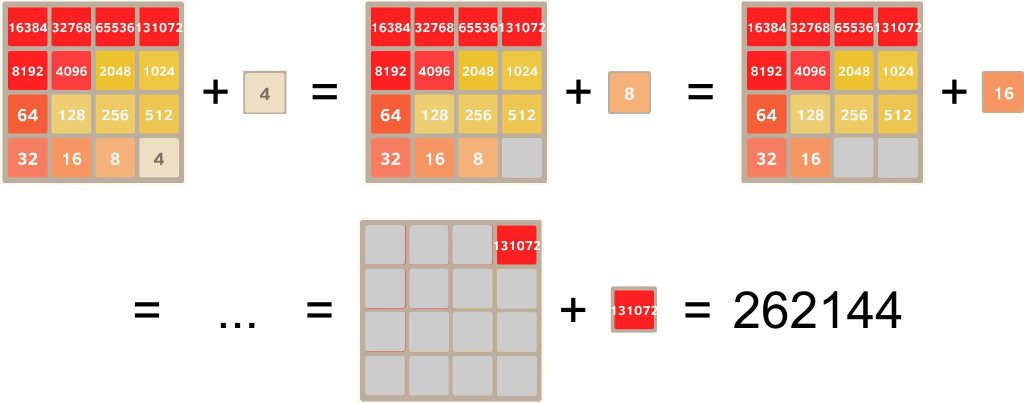
\includegraphics[width=1.0\textwidth]{Sum-of-All-Tiles.png}
            \caption{Mathematical End of the 2048}
            \label{cMathematical_End_of_2048}
        \end{figure}

    \end{itemize}
    \todo{Expectimax algo is too big. Need to reduce text in it}
    \begin{algorithm}[h!]
        \SetAlgoLined
        \Function{get\_moves}{board\_state}
        \State For each move perform \textbf{EXPECTIMAX\_SEARCH(board\_state, depth=4)} and evaluate future configurations of the board recursively for depth 4 \\
        \State Store the fitness value for each move in \textit{moves\_fitness\_dictionary} \\
        \Return \textit{moves\_fitness\_dictionary}
        \EndFunction

        \Function{evaluation}{board\_state}
        \State Calculate the fitness of the board\_state by flattening the board to implement Snake-Line Pattern heuristics and multiply each term of the sequence with a term in geometric series\\
        \State Penalize the board that does not have highest valued tile in the lower left corner of the board\\
        \Return \textit{fitness}
        \EndFunction

        \Function{Expectimax\_Search}{board\_state, depth, is\_AI\_move = False}
        \State \If{ depth == 0 or no\_move\_exists() }{ \State \Return  \textbf{EVALUATION(board\_state)}}
        \State Calculate fitness using \textbf{EVALUATION(board\_state)}\\
        \State \uIf{ is\_AI\_move}{
            \State Store the fitness values of each child board\_state generated after performing recursive \textbf{Expectimax\_Search(child\_board\_state ,depth-1)} for all possible moves\\
        }
        \State \Else{
            \State For every empty position in the board spawn two childern \State board\_states (board with a new 2-tile and a new 4-tile \State respectively)\;
            \State Return weighted (as per 90:10 Distribution) average of the fitness \State of every  child generated after performing recursive \State \textbf{Expectimax\_Search(child\_board\_state ,depth-1)}
        }
        \Return \textit{fitness}
        \EndFunction


        initialize\_gamegrid()\;
        \While{True}{
            Get the moves\_fitness\_dictionary for current board\_state using \textbf{GET\_MOVES(board\_state)}\;
            play the move from moves\_fitness\_dictionary with maximum fitness\;
            \If{ no\_move\_exists() }{Stop}
        }
        \caption{Expectimax Search Algorithm}
    \end{algorithm}

    \subsection{Q Learning}

    Q-Learning is a reinforcement learning algorithm \cite{watkins1992q}. A Q-Learning agent makes actions that are outside of the current policy. As such it is considered an 'off-policy' reinforcement learning algorithm. We used Q-learning to experiment with how well reinforcement learning could work with a problem such as 2048. For this we created a Deep Q Network (DQN) based on the works by \cite{dqnGit}.

    The model is trained using Tensorflow. It consists of 2 convolution layers, an expansion, and a hidden layer. The first convolution layer consists of 2 convolution 2D tensors, while the second layer uses 4 tensors. The expansion and hidden layer reshapes the output to the required form.

    The model was trained with Gamma and Epsilon values of 0.9, and the starting learning rate is set as 0.0005. The replay memory is initialized with 6 GB of memory which is used to sample the minibatch. A RELU activation function was used with an RMSProp optimization function. The Epsilon value is used as a threshold to use greedy approach randomly, hence . After certain intervals, the epsilon value is further reduced. The learning rate also decays exponentially by each episode. The model is trained for 20,000 episodes.

    \begin{algorithm}[h!]
        \SetAlgoLined
        Initialize hyperparameters and replay memory\;
        Initialize action value function Q with random weights\;
        \For{episode in 1 to M}{
            Initialize 2048 board
            \While{game is not lost}{
                \eIf{epsilon $>$ random value}{
                    Set up temporary board \\
                    Use greedy approach to take action and observe reward \\
                    Make the action with max reward on the real board \\
                }{
                    Find moves with the max Q value\\
                    \For{control in Q value table}{
                        Set up temporary board\\
                        Take control action and observe reward \\
                    }
                    Make the action with max reward on the real board \\
                }
                Store observations in replay memory \\
                \If{replay memory $>$ memory limit}{
                    Back-propagate and sample the mini batch\\
                    Store layer weights
                }
                Reduce epsilon and learning rate values\\
            }
        }
        \caption{DQN Algorithm}
    \end{algorithm}

    \section{Experimental Results}
    In this project, the game simulations are carried out using TKinter library in python \cite{Tkinter}. The  running game environment setup is referenced from the following source\cite{yangshun}.
    Further, each algorithm is simulated over the same environment. The README.md from the project repository \cite{AI-RKRS} has instructions for setting up the local environment and running implemented algorithms in the 2048 game. It also contains evaluation source files in csv format.

    Table \ref{depth-analysis} captures the performance analysis of Expectimax alogrithm for different depth limits. It has been observed that the Expectimax search approach achieves a max tile of 2048 at depth 2 by performing 1460 moves. To assess the performance of the Expectimax search we also ran the simulation 10 times at depth 4 and could achieve the 4096 tile more than 60\% of the time.
    According to figure \ref{comparative_analysis_of_algorithms}, Expectimax algorithm in its default configuration of depth 1 and 400 limited moves outperforms rest of the AI approaches.
    \begin{table}[t]
        \centering
        \caption{Expectimax Search: Depth Analysis}
        \label{depth-analysis}
        \begin{tabular}{|c|c|c|c|c|}
            \hline
            Depth & Max-Tile & Moves & score & Execution Time (min)\\
            \hline
            1 & 256  & 238  & 2804   & 0.03   \\
            2 & 2048 & 1460 & 27844  & 0.29   \\
            3 & 2048 & 1862 & 35932  & 1.25   \\
            4 & 8192 & 5594 & 132780 & 31.65 \\
            \hline
        \end{tabular}
    \end{table}



    \subsection{Methodology}
    Greedy First, MCTS and Expectimax algorithms are evaluated and compared based on the Max Score and Average score achieved for 100 consecutive runs. The agent is allowed to perform 400 moves in each indivual run. Further, the average score and max score is compared using bar chart as shown in Figure \ref{comparative_analysis_of_algorithms}. Also, the Game Progression Chart shown in Figure \ref{game_score_progression_chart} demonstrates how an individual algorithm is able to score as game progresses.
    \todo{@Rohan add Methodology for DQN}
    For our DQN Agent, we analyze its scores over the number of episodes we trained it for.

    We use a depth limited Expectimax Search approach to solve the 2048 problem in polynomial time. Since we take a weighted average of all children nodes obtained in the depth limited recursive search, we did not apply alpha-beta pruning \cite{7162574} to get rid of the branches thus reducing the search space.


    \subsection{Results}

    Figure \ref{comparative_analysis_of_algorithms} shows that Expectimax algorithm outperformed all the implemented algorithms while Random Moves algorithm sets a baseline for comparison. Greedy Algorithm performed well when compared with MCTS with all heuristics variations. Three variations of heuristic functions mentioned in section \ref{heuristics} are used and its performance in Greedy First algorithm and MCTS algorithm is measured. From game score, it is clear that Empty Cell Heuristics performed better than weighted cell heuristics.

    Figure \ref{game_score_progression_chart} captures progression of game score in individual runs of implemented algorithms. In Random moves algorithm, the game got over in nearly first 100 moves, whereas gameplay of Expectimax algorithm is still in progression even after performing 400 moves. This chart provides an overview of how game progresses and number of steps around which it gets over.

    \begin{figure}[h!]

        \centering
        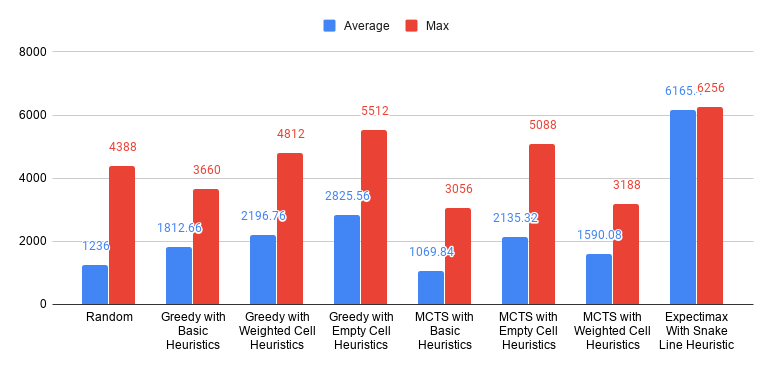
\includegraphics[width=1.0\textwidth]{Comparative Analysis.png}
        \caption{Comparative Analysis of Algorithms}
        \label{comparative_analysis_of_algorithms}
    \end{figure}

    \begin{figure}[h!]

        \centering
        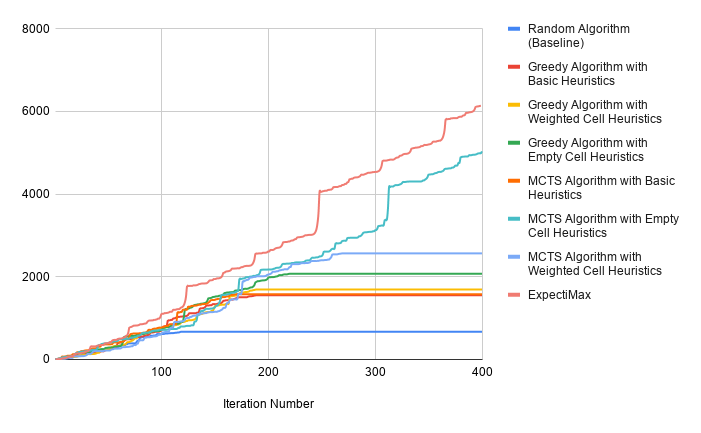
\includegraphics[width=1.0\textwidth]{Game Score Progression Chart.png}
        \caption{Game Score Progression Chart}
        \label{game_score_progression_chart}
    \end{figure}

    \subsection{Interpretations}
    The greedy first approach is definitely better than a random move approach but its not always the case.
    Consider the following situation,
    \begin{figure}[h!]

        \centering
        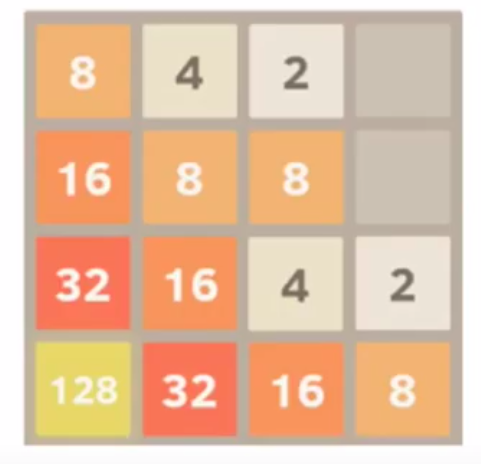
\includegraphics[width=0.15\textwidth]{greedy_img_correction.png}
        \caption{Demonstration of a game state when Greedy approach fails}
    \end{figure}


    The greedy first approach will take \textbf{LEFT} action in order to increase the final game score. In such cases, swiping \textbf{UP} then swiping \textbf{LEFT} is a better than swiping \textbf{LEFT} in the first place. In order to improve the greedy first algorithm, we introduce heuristics which helps agent take appropriate action based on the strategies and rewards assigned for the chosen strategy.

    One of the reason, Greedy Approach performed well as compared to MCTS could be that, the Play-out happens randomly in MCTS algorithm. The level of randomness is more in MCTS when compared with Greedy approach.




    \section{Conclusions}
    There is an uncertainty in the 2048 game. The randomly generated new tiles of each stage create an uncertain environment.

    \subsection{Improvements}
    \begin{itemize}
        \item \textbf{Improving the Speed:} Improving the speed of the algorithm will allow you to use larger depth and thus get better accuracy. Storing gamegrid in the form of bitvector will help save memory and in turn it can improve the performance.

        \item \textbf{Tuning Heuristics:} In the current implementation, only one heuristic is considered at a time by controlling alpha, beta, gamma from equation. In future, combination of several heuristics using weighted coefficients can be used. Several implementation mentions the use of  Monotonicity and Smoothness of gamegrid for heuristic calculation which can be examined. Experimenting more with heuristics can reveal different ways in which gameplay can be improved.

    \end{itemize}

    \bibliography{ai_doc}
    \bibliographystyle{ieeetr}

\end{document}
